\documentclass[a4paper,twoside,kulak]{kulakreport}



\usepackage[dutch]{babel}
\usepackage{hyperref}
\usepackage{graphicx}
\usepackage{flafter}
\usepackage{amsmath, amssymb, amsthm}
\usepackage{siunitx}
\usepackage{pdfpages}
\usepackage{subfiles}
\usepackage{wrapfig}
\usepackage{float}
\usepackage{url}
\usepackage{translator}
\usepackage{pdfpages}

\uselanguage{Dutch}
\usepackage{longtable}
\usepackage{booktabs}
\usepackage{enumitem}
\usepackage{array}
\providetranslation[to=Dutch]{Figure}{Figuur}

\usepackage{etoolbox}
\usepackage{booktabs}
\usepackage{xstring}
\usepackage{xcolor,colortbl}
\definecolor{gray1}{gray}{0.7}
\definecolor{gray2}{gray}{0.85}
\definecolor{gray3}{gray}{0.95}

% counting system		
\newcounter{counter}
\newcounter{subcounter}
\newcounter{subsubcounter}
\newcommand{\teller}{
	\stepcounter{counter}
	\setcounter{subcounter}{0}
	\setcounter{subsubcounter}{0}
	\thecounter}
\newcommand{\subteller}{
	\stepcounter{subcounter}
	\setcounter{subsubcounter}{0}
	\thecounter.\thesubcounter}
\newcommand{\subsubteller}{
	\stepcounter{subsubcounter}
	\thecounter.\thesubcounter.\thesubsubcounter}

% row	
\newcommand{\row}[3]{
	\IfEqCase{#1}{
		{1}{\teller & #2 & \IfEqCase{#3}{{0}{niet OK}{1}{OK}} \\}
		{2}{\subteller & #2 & \IfEqCase{#3}{{0}{niet OK}{1}{OK}} \\}
		{3}{\subsubteller & #2 & \IfEqCase{#3}{{0}{niet OK}{1}{OK}} \\}
	}[PackageError{row}{Undefined option to row: #1}]}





\faculty{Groep Wetenschappen \& Technologie}
\group{\texttt{X0B54a} -- Probleemoplossen en ontwerpen, deel 2}
\title{Ontwerpproces van een zelfrijdende wagen}
\subtitle{Tussentijds verslag}
\author{Team 4: Team R2D2}
%\emailaddress{}
\institute{Matthijs Deforche, Karl Van Holder, Thomas Varheust, Kobe De Weerdt, Yaron Verhulst}
\date{Academiejaar 2020 -- 2021}
\address{\textbf{\theauthor}\\
	Groep Wetenschap \& Technologie \\
	KU Leuven Kulak           \\
	Etienne Sabbelaan 53, 8500 Kortrijk
}

\begin{document}
	\titlepage
	
	\chapter*{Abstract}
	
	\renewcommand*\contentsname{Inhoud}
	\tableofcontents
	
	\chapter*{Lijsten van tabellen en figuren}
	\section*{Figuren}
	\begin{itemize}
		\item \ref{fig: lijnvolg}: Visualisatie van het principe van ons lijnvolgalgoritme.
		\item \ref{fig: verkeerslicht}: Technische tekening verkeerslicht, opgehaald van \cite{artikel1}
		\item \ref{fig: kruispunt}:Bovenaanzicht kruispunt met relevante maten en items, aangepast vanuit \cite{Smart}. 
		\item \ref{fig: wagen}: CAD-ontwerp van de wagen, samengesteld uit \textit{.par-onderdelen}, gezien vanuit de rechterbovenhoek.
		\item \ref{fig: skelet}: Het 3D-geprinte onderdeel \textit{Skelet van de wagen}.
		\item \ref{fig: fchart}: De flowchart van ons algortime
		
		\item \ref{fig: pie}: Visualistie van de besteding van ons budget.
		
		
	\end{itemize}

	\section*{Tabellen}
	\begin{itemize}
		\item \ref{tab: taken}: Takenstructuur
		\item \ref{tab: ess}: Uitgaven hardware
		\item \ref{tab: ontw}: Uitgaven ontwerp
		\item \ref{tab: ass}: Uitgaven assemblage
		\item \ref{tab: onk}: Uitgaven onkosten
	\end{itemize}
	
	
	\chapter*{Inleiding}

Wij zijn vijf studenten ingenieurswetenschappen in het eerste jaar aan de Katholieke Universiteit Leuven Campus Kulak Kortrijk.
Het vak P\&O 1 en de andere vakken van het eerste semester hebben ons de nodige kennis gegeven om het vak P\&O 2 aan te vatten. 
De opzet van de teamopdracht dit semester is een zelfrijdend wagentje te ontwerpen en te bouwen dat uiteindelijk zelfstandig door een modelstad zal moeten rijden. Het wagentje moet niet alleen kunnen rijden, ook moet het obstakels zoals tegenliggers en voorgangers kunnen detecteren. Het wagentje zal kruispunten en verkeerslichten correct moeten  interpreteren en zal er gepast op reageren. Het ontwerpen en het bouwen van het wagentje kan met behulp van een virtueel budget, een interface LABVIEW om met het wagentje te kunnen communiceren, een CAD-programma om onze wagen te 3D-modelleren enz. 
Een extra toevoeging aan de opdracht is om onze wagen een persoonlijke touch te geven. 
	
	%%hoofdtekst
	\chapter{Methodologie}
	
	
	
	\section{Planning}
	
	Voor de planning van onze teamopdracht hebben we enkele tools gebruikt die in de volgende secties uitgelegd zullen worden. 
	\subsection*{Klantenvereisten}
	Eerst en vooral hebben we de klantenvereisten opgesteld. De opdracht die we kregen bevat alle informatie van wat er tegen het eind van het project van ons verwacht wordt. Om hier het overzicht in te bewaren, hebben we de klantenvereisten opgesteld. Per item hebben we een klantenvereiste opgesteld die een algemene beschrijving hiervan is. De klantenvereisten zijn terug te vinden in bijlage \ref{seq: klantver}. 
	
	\subsection*{Ontwerpspecificaties}Aan de hand van deze klantenvereisten hebben we de ontwerpspecificaties samengesteld. Een klantenvereiste is eerder algemeen terwijl de ontwerpspecificaties veel gedetailleerder zijn. Door de ontwerpspecificaties op te stellen, hebben we nu een beter en duidelijker beeld van hoe een klantenvereiste ineen zit.De ontwerpspecificaties zijn terug te vinden in bijlage \ref{sec: ontws}. 
	
	\subsection*{Teamverantwoordelijkheden}De teamopdracht vergt een goede planning en een goede werkverdeling. Daarom hebben we per categorie een tweetal studenten verantwoordelijk gesteld. Met een categorie bedoelen we bijvoorbeeld programmeren, Solid Edge enzovoverder. De teamverantwoordelijkheden zijn terug te vinden in bijlage \ref{seq: vera}.
	 
	\subsection*{Takenstructuur}Om het werk te verdelen onder elkaar hebben we een takenstructuur gemaakt. Deze bevat alle deeltaken die nodig zijn om ons project tot een goed einde te brengen. De deeltaken zijn verdeeld onder een samenvattende hoofdcategorie. Bijvoorbeeld bij de categorie Solid Edge is er een deeltaak 'wiel modelleren'. De takenstructuur is terug te vinden in bijlage \ref{sec: taken}.
	\subsection*{Gantt-grafiek \& Teamkalender} Nu we de verschillende deeltaken hebben opgesteld is het mogelijk om deze in te plannen. We hebben de deeltaken genummerd en een teamkalender opgesteld om te plannen wanneer een deeltaak afgewerkt moet zijn. Het nummer van de deeltaak wordt bij de week/dag geplaatst wanneer het af moet zijn in de teamkalender. Een teamkalender vertelt echter niet hoeveel tijd een deeltaak in beslag zal nemen. Daarom hebben we een bijhorende Gantt-grafiek gemaakt. Deze toont per deeltaak hoeveel tijd we eraan zullen besteden. Wanneer een deeltaak pas kan aangevat worden als een andere deeltaak is afgewerkt, zullen we dit in de Gantt-grafiek aanduiden met een pijl. De Gantt-grafiek en Teamkalender zijn terug te vinden in bijlage \ref{sec: kale}.
	
	\section{Ontwerp}
	\subsection{Onderdelen}
		We kozen voor de NI Myrio-microcontroller omdat deze het simpelste is en voor de aard van de opdracht voor ons het efficiëntste leek. Bovendien hebben we via de NI Myrio altijd een handige visualisatie van het programma en kunnen we gebruik maken van de analoge afstandssensor die met een bereik van 10 to 80 centimeter de meest geschikte afstandssensor is.
	Door deze keuze kunnen we voor de andere sensoren enkel de analoge versie gebruiken. Aangezien de NI Myrio een power input nodig heeft van 6-16 Volt, kan de powerbank niet gebruikt worden. Door 2 Lithium-ion batterijen van $3,6$ Volt te kiezen en deze in serie te schakelen is het wel mogelijk om een geschikte power-input te verkrijgen.
	Als persoonlijke touch kozen we om geen makerbeams te gebruiken. Hierdoor leek het ons het beste om een groot chassis te hebben. We kozen het rechthoekig zwart boven het universeel chassis omdat ze redelijk gelijkaardig zijn, maar het universeel chassis 50 eenheden meer kost. Om dit chassis stabiel te maken kozen we ervoor om de ball caster te gebruiken samen met 2 aangedreven wielen. Als wiel kozen we voor de wielen met een breedte van 8 millimeter en diameter van 60 millimeter, deze zijn de grootste en kunnen samen met de spacers van de ball caster ervoor zorgen dat het chassis perfect horizontaal ligt. Als aandrijving hadden we de voorkeur voor de "Micro Metal Gear Motor 50:1 HP". Deze heeft een 3 millimeter as, wat compatibel is met onze gekozen wielen en heeft een gemiddeld vermogen om de wagen te doen stoppen en opnieuw te versnellen. Omdat deze motoren niet meer beschikbaar waren wanneer wij onze bestelling konden plaatsen kozen we voor de "Micro Metal Gear Motor 100:1 HP", deze is redelijk gelijkaardig maar heeft een ander vermogen. Samen met deze motoren kozen we 2 motorbeugels om de motoren aan het chassis te kunnen bevestigen en de "Dual Drive DRV8833" zodat we beide motoren tegelijk kunnen aansturen.
	Om eerst de wagen te testen voor we gaan solderen op de printplaat kozen we nog een breadbord, aangezien we maar 3 sensoren en 2 motoren hadden kozen we voor het kleinere formaat omdat dit ons minder budget kost. 
	\subsection{Assemblage}
	Om de poorten van de myRIO-microcontroller vrij te houden, hebben we de myRIO boven de wielen geplaatst. Omdat de myRIO relatief zwaar is ten opzichte van de andere onderdelen, zorgt deze keuze ervoor dat het zwaartepunt van de wagen hoger komt te liggen. Om te voorkomen dat het zwaartepunt te hoog zou liggen, plaatsten we de batterijen centraal op het chassis. De reflectie sensor wordt vooraan in het verlengde van het chassis bevestigd via de "reflectie sensor houder", een onderdeel dat we zelf ge-3D-print hebben omdat we ervoor gekozen hebben om geen makerbeams te gebruiken. De technische tekening van de \textit{reflectie sensor houder} is terug te vinden in bijlage \ref{sec: vis}. Omdat de afstandssensor maar objecten waarneemt vanaf 80mm hebben we besloten deze op 35mm van de voorkant van het chassis te plaatsen, zo kan deze efficiënter gebruikt worden. De kleurensensor wordt op 75mm boven de grond, 25mm horizontale afstand van de reflectie sensor en op 65mm van de symmetrieas van het chassis omdat het zich zo op de ideale positie bevindt om het verkeerslicht uit te lezen wanneer de auto stilstaat. De afstandssensor en kleurensensor worden geïntegreerd in de wagen via het \textit{Skelet van de wagen}, dit is een ge-3D-print onderdeel die ook de myRIO ondersteunt en waarvan een afbeelding te zien is in figuur \ref{fig: skelet} in bijlage \ref{sec: vis}. De sensoren maken verbinding met de myRIO via de printplaat, deze is via plakband bevestigd op de myRIO zodat er voldoende ruimte is om overzichtelijk alles te bevestigen. Het elektrisch circuit is te zien in bijlage \ref{sec: circ}. Het 3D-model van de wagen is te zien in figuur \ref{fig: wagen} in bijlage \ref{sec: vis}.
	
	
	\section{Implementatie}

	\subsection{Implementatie software}
	Als microcontroller hebben wij voor de MyRio gekozen, omdat het ons eenerzijds handiger leek om direct alles in LabVIEW te programmeren dan enkel de interface in LabVIEW te maken. Anderzijds ook omdat we de analoge afstandssensor liever wilden gebruiken dan de digitale (ze hebben een andere range).
	
	\subsection{Algoritmen}
	Voordat we begonnen met programmeren bedachten we eerste welke functies de auto zou moeten kunnen uitvoeren.\\
	We kwamen tot volgende functies:
	\begin{itemize}\item De auto moet een zwarte lijn kunnen volgen en zich corrigeren als de auto wat afwijkt van de baan.
		\item Terwijl de auto de lijn volgt moet hij ook voorliggers kunnen detecteren en vertragen wanneer de afstand te klein wordt.
		\item De auto moet kunnen stoppen aan een stoplijn en daarvoor moet hij een gematigde snelheid hebben.
		\item Wanneer de auto stopt voor een kruispunt moet hij het verkeerslicht herkennen en hier gepast op reageren.
		\item De auto moet kunnen inslaan op een kruispunt en bij een bocht.
		\item De auto moet op ieder moment extern bestuurd kunnen worden.\end{itemize}
	
	
	\subsection{Lijnvolgalgoritme}
	Op de baan die de robot moet volgen zijn allemaal donkere lijnen getrokken. Bij het volgen van deze lijnen maken we gebruik van de "QTR-8A analoge reflectie sensor array".
	De aansluiting hiervan op de microcontroller kan je zien in bijlage \ref{sec: circ}. De sensor heeft 8 lichtgevoelige sensoren. We hebben ons lijnvolgalgoritme gebaseerd op het feit dat men aan de ene kant van de sensor meer zwart ziet dan aan de andere wanneer die niet evenwijdig met de lijn rijdt. Wanneer men meer zwart ziet aan de linkerkant van de sensor, moet men naar links draaien (dit door de linkermotor trager te doen draaien). Wanneer men echter meer zwart ziet aan de rechterkant van de sensor, moet men naar rechts draaien (dit door de rechtermotor trager te doen draaien ). Als men aan beide zijden even veel zwart detecteert moet men rechtdoor blijven rijden. Dit alles kan men ook zien in  \ref{fig: lijnvolg}. Dit algortime komt tot een einde wanneer beide kanten even veel zwart ervaren en deze waardes tesamen veel groter zijn. Dit betekent dat er een stopstreep is, en men dus moet stoppen. 
	
	\begin{figure}
		\centering
		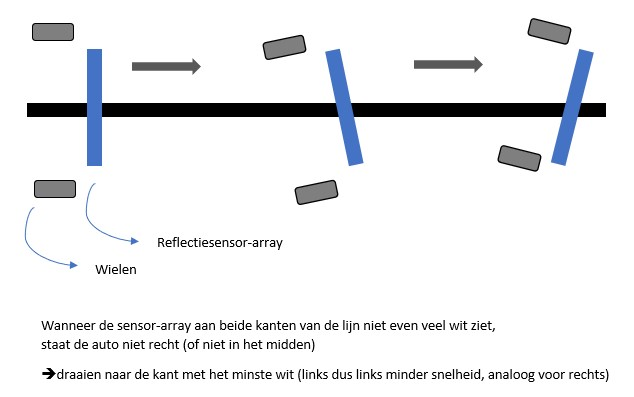
\includegraphics[width=.84\textwidth]{pref2}
		\caption{Visualisatie van het principe van ons lijnvolgalgoritme.
		}
		\label{fig: lijnvolg}
		
	\end{figure}
	\subsection{Licht herkennen}
	Dit algoritme treedt pas in werking als men een stopstreep detecteert. Dit is zo wanneer de 8 sensoren van de reflectiesensor zwart detecteren (zoals in vorige paragraaf beschreven). Met behulp van een while-loop gaan we kijken of het licht groen is dat de kleurensensor detecteert. We gaan gebruik maken van een polling rate van 1 seconde zodat we de myRIO niet overbelasten. Zolang het rood is blijft de while-loop lopen, vanaf de kleurensensor groen ziet, stopt die while-loop en kan het traject verdergezet worden.
	
	\subsection{Andere wagen herkennen en versnellen/vertragen}
	
	Met de afstandssensor kunnen we de afstand tot een voorliggende wagen detecteren. Wanneer de afstand te klein is, gaat de wagen vertragen. Om dit te implementeren  maken we gebruik van een while-loop. Als echter bij het vertragen de kritieke minimale snelheid overschreden wordt(dus nog minder dan de minimale), dan stopt onze wagen(dit is wanneer een andere wagen voor ons stilstaan). Versnellen gebeurt ook met een while loop, wanneer de snelheid boven een bepaalde waarde is, neemt hij de 'ideale snelheid' aan.
	
	\subsection{Draaien op kruispunt}
	We maken een ondersheid tussen 3 gevallen; linksaf, rechtsaf en rechtdoor. Bij linksaf moeten we eerst 375mm rechtdoor rijden, dan 90graden naar links draaien om de as van de wagen en tenslotte meer dan 375 mm rechtdoorrijden om dan weer de lijn te volgen.
	
	Bij rechtsaf moet men eerst 125mm rechtdoorrijden, dan 90graden naar rechts draaien om de as van de wagen en tenslotte meer dan 125mm rechtdoorrijden om dan weer de lijn te volgen. Bij rechtdoor moet men meer dan 500mm rechtdoorrijden om dan vervolgens de lijn te volgen. bij deze drie gevallen moet men tijdens het uitvoeren ervan rekening houden of er al dan niet een voorligger zich binnen de zeer kritische gevarenzone bevindt (dit wil zeggen dat de ander wagen voor de een of andere reden stilstaan op het kruispunt)
	
	\subsection{Manual override}
		Om de controle manueel over te nemen sturen we de motoren rechtstreeks aan. Dit stellen we voor met behulp van twee sliders in LabVIEW. Later zullen we aan die sliders concreet een invulling voor geven om op de test te gebruiken.
	
	\subsection{Implementatie traject}
	
	Vanaf het moment dat we ons traject kennen, kunnen we aan de hand van de vorige algoritmes ons parcours samenstellen. De flowchart van ons programma is terug te vinden in bijlage \ref{sec: flowchart}.
	
	\subsection{Concrete implementatie}
	Het hele LabVIEW programma, gebruikmakend van de voorgenoemde functies in de vorm van subVI's, splitsen we op in twee stappen:\bigskip
	
	De eerste stap is het rijden. Hier moet de auto tegelijk de lijn op de grond volgen, een goede afstand tot zijn voorligger behouden (wat dus inhoudt dat die de voorligger moet detecteren en aan de hand van de afstand tot die voorligger zijn snelheid moet aanpassen) en de auto moet ook nog eens comfortabel kunnen stoppen wanneer die een stopstreep detecteert. Al deze inputs komen van de sensoren aan boord van de auto.\bigskip
	
	De tweede stap hier begint bij die stopstreep. Wanneer de auto gestopt is aan de stopstreep moet die een verkeerslicht detecteren en daar gepast op reageren, nadat het groen licht geworden is moet die dus over het kruispunt draaien. Daarna moet die een bocht nemen of rechtdoor rijden aan de hand van een vooraf opgesteld parcours. Na deze stappen is het algoritme klaar en begint hij weer met stap 1.\bigskip
	
	Op het moment van dit verslag zijn we zo goed als klaar met het schrijven van LabVIEW-functies om deze taken te vervullen en moet slechts geïmplementeerd worden hoe we de inputs van de sensoren bij de LabVIEW-programma's kijgen en daarna ook de outputs van onze programma’s bij de motoren krijgen.
	
	
	\chapter{Resultaten}
	
	\section{Budget}
	Een financieel verslag is terug te vinden in bijlage \ref{sec: finrap}.
	
	\chapter{Discussie}
	%%besluit
	\chapter{Bijlagen}
	\section{Planning}
	\label{sec: planning}
	
	\providetranslation[to=Dutch]{Figure}{Figuur}
	
	
	
	\setlist[itemize]{noitemsep, topsep=0pt, leftmargin=*}
	\uselanguage{Dutch}

	\providetranslation[to=Dutch]{Figure}{Figuur}
	
	
	
	\section{Overzicht ontwerpspecificaties}
	\label{sec: ontws}
	De verkeerslichten kunnen interpreteren: stoppen bij een rood licht, doorrijden bij een groen licht:\\
	De hoogte van het verkeerslicht gemeten vanaf de grond tot aan het middelpunt van het verkeerslicht is $75mm$. Het verkeerslicht heeft een knipperfrequentie van $1Hz$. Een technische tekening van het kruispunt is te zien op \ref{fig: verkeerslicht}.
	\bigskip
	
	
	
	Een geïmplementeerd traject kunnen volgen / stoplijn detecteren:\\
	De ondergrond van het traject zal ofwel donker ofwel helder zijn. De kleur van de lijnen die de auto moet volgen zal afhangen van wat de kleur van de ondergrond is. Het zal het omgekeerde zijn waardoor het verschil duidelijk is. Er zijn ook nog verschillen in de soorten lijnen die op de ondergrond aangebracht zullen worden. De breedte van een volglijn is $25mm$ en de breedte van een stoplijn is $50mm$. De kruispunten liggen op $1000mm$ van elkaar en figuur \ref{fig: kruispunt} toont het bovenaanzicht van een kruispunt. 
	
	
	\bigskip
	
	
	Commando's van een computer kunnen volgen:\\
	Vooraleer onze auto het traject mag oprijden, moeten we eerst op afstand een noodstop kunnen uitvoeren. 
	
	
	
	\bigskip
	
	De auto moet aan een bepaald budget voldoen:\\
	Er is een budget van $3500$ eenheden beschikbaar. Dit budget kunnen we gebruiken om materiaal aan te kopen op de site: http://www.irkulak.be/po2/.
	Verder kunnen we het budget ook nog gebruiken om onze eigen ontwerpen te 3D-printen. 
	
	\bigskip
	Het volledige traject foutloos kunnen afleggen met een aanvaardbaar tempo:\\
	De wagen heeft een maximumbreedte van $250mm$, een maximumhoogte van $300mm$ en een minimumhoogte van $75mm$.
	
	\bigskip
	
	\begin{figure}
		\centering
		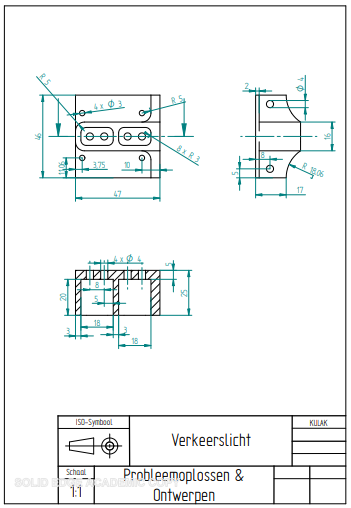
\includegraphics[width=.8\textwidth]{verkeerslicht}
		\caption{Technische tekening verkeerslicht, opgehaald van \cite{artikel1}. }
		\label{fig: verkeerslicht}
	\end{figure}
	\bigskip
	\begin{figure}
		\centering
		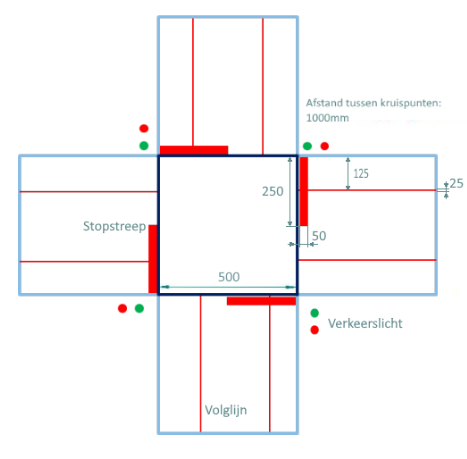
\includegraphics[width=.8\textwidth]{bovenaanzichtkruispunt}
		\caption{Bovenaanzicht kruispunt met relevante maten en items, aangepast vanuit \cite{Smart}.
		}
		\label{fig: kruispunt}
		
	\end{figure}
	\section{Samenvatting klantenvereisten}
	\label{seq: klantver}
	Voor de bouw van ons wagentje zijn er meerdere vereisten waar we rekening mee moeten houden. Dit document is een samenvatting hiervan.\\
	
	De constructie van onze wagen moet aan een bepaald budget voldoen van 3500 eenheden. Er is een materiaallijst beschikbaar die we kunnen raadplegen om onderdelen te bestellen. \\
	
	Onze auto moet een geïmplementeerd traject kunnen volgen via een lijn die op de ondergrond is aangebracht. Deze verschilt qua intensiteit met de ondergrond zodat de auto de lijn kan herkennen. Het traject bevat ook meerdere kruispunten met verkeerslichten. Onze auto moet deze kunnen interpreteren en gepast reageren op het rode of groene licht. Om te kunnen stoppen bij het rode licht zal onze auto een dikke stoplijn moeten kunnen detecteren. \\
	
	Om het traject te volgen zal onze auto dus moeten kunnen rijden en draaien. Ook stoppen is belangrijk. Onze auto moet namelijk voorliggers kunnen detecteren en op tijd stoppen om een botsing te vermijden. Er wordt verwacht dat het volledige traject foutloos uitgereden kan worden op een aanvaardbaar tempo. \\
	
	Voor onze auto het traject op kan, zullen we ook een noodstop moeten uitvoeren. Dit zal via commando's van een computer moeten gebeuren.
	
	\bigskip
	
	\section{Teamverantwoordelijkheden}
	\label{seq: vera}
	\includepdf[pages=6]{Team4_planning.pdf}
	
	\section{Takenstructuur}
	\label{sec: taken}
	
			
		\begin{table}
			\centering
			%\caption{Takenstructuur}
			
			Tabel 1: Takenstructuur
			
			% \vspace{\baselineskip}
			\begin{tabular}{p{1cm}p{12cm}c}
				
				
				\toprule
				Code & Taak & Status \\ 
				
				\midrule
				\row{1}{Inwerken}{1}
				\row{2}{Documenten op Toledo lezen}{1}
				
				\row{2}{Ontwerpen en plannen}{1}
				\row{3}{Materiaallijst maken}{1}
				\row{3}{Teamkalender maken}{1}
				\row{3}{Klantenvereisten opstellen}{1}
				\row{3}{Overzicht ontwerpspecificaties}{1}
				\row{3}{Takenstructuur}{1}
				\row{3}{Gantt-grafiek}{1}
				
				\midrule
				\row{1}{Ontwerpen met behulp van de computer}{0}
				\row{2}{3D modellen	(Solid parts)}{1}
				\row{3}{Wiel}{1}
				\row{3}{Motor}{1}
				\row{3}{Motorbeugel}{1}
				\row{3}{Chassis}{1}
				\row{3}{Ballcaster}{1}
				\row{3}{Printplaat}{1}
				\row{3}{Kleursensor}{1}
				\row{3}{Afstandssensor}{1}
				\row{2}{Assemblage (Assembly)}{1}
				
				
				\row{2}{Technische tekeningen (Drawing)}{0}
				
				\row{2}{Stuklijst}{0}
				
				\midrule
				\row{1}{Software}{0}
				\row{2}{Sturen/snelheid regelen}{1}
				\row{2}{Lijnvolgalgoritme}{1}
				\row{2}{Verkeerslichtinterpretatie}{1}
				\row{2}{Voorliggerdetectie}{1}
				\row{2}{Stoppen}{1}
				\row{2}{Vertragen}{1}
				\row{2}{Handmatig besturen}{1}
				\row{2}{Inputs vormgeven}{0}
				\row{2}{Outputs vormgeven}{0}
				\row{2}{Testen}{0}
				
				
				\midrule		
				\row{1}{Rapportering}{0}
				\row{2}{Tussentijds verslag}{1}		
				\row{3}{Nalezen}{1}
				\row{2}{Tussentijdse presentatie}{0}
				\row{3}{Structuur}{1}
				\row{3}{Presentatie maken}{0}
				\row{3}{Nalezen}{0}
				\row{3}{Inoefenen}{0}
				\row{2}{Eindverslag}{0}
				\row{3}{Structuur}{0}			
				\row{3}{Nalezen}{0}
				\row{2}{Eindpresentatie}{0}
				\row{3}{Structuur}{0}
				\row{3}{Presentatie maken}{0}
				\row{3}{Nalezen}{0}
				\row{3}{Inoefenen}{0}
				\bottomrule
			\end{tabular}
		\caption{Takenstructuur}
		\label{tab: taken}
		\end{table}
	\newpage
	
	
	\section{Gantt-grafiek \& Teamkalender}
	\label{sec: kale}
	\includepdf[pages = 7]{Team4_planning}
	\includepdf[pages = 8]{Team4_planning}
	\includepdf[pages = 9]{Team4_planning}
	\includepdf[pages = 10]{Team4_planning}
	\includepdf[pages = 11]{Team4_planning}
	\includepdf[pages = 12]{Team4_planning}
	\includepdf[pages = 13]{Team4_planning}
	
	
	
	\section{Visualisatie ontwerp}
	\label{sec: vis}
	
\begin{figure}[h]
		\centering
		\includegraphics[width=1.2\textwidth]{KS®wagen1.3}
	\caption{CAD-ontwerp van de wagen, samengesteld uit \textit{.par-onderdelen}, gezien vanuit de rechterbovenhoek.}
		\label{fig: wagen}
\end{figure}

\begin{figure}[h]
	\centering
	\includegraphics[width=1.2\textwidth]{KS®skelet.4}
	\caption{Het 3D-geprinte onderdeel \textit{Skelet van de wagen} }.
	\label{fig: skelet}
\end{figure}
%%KS®wagen1.3

\section{Elektrisch circuit}
\label{sec: circ}

\section{Flowcharts}
\label{sec: flowchart}

\begin{figure}
	\centering
	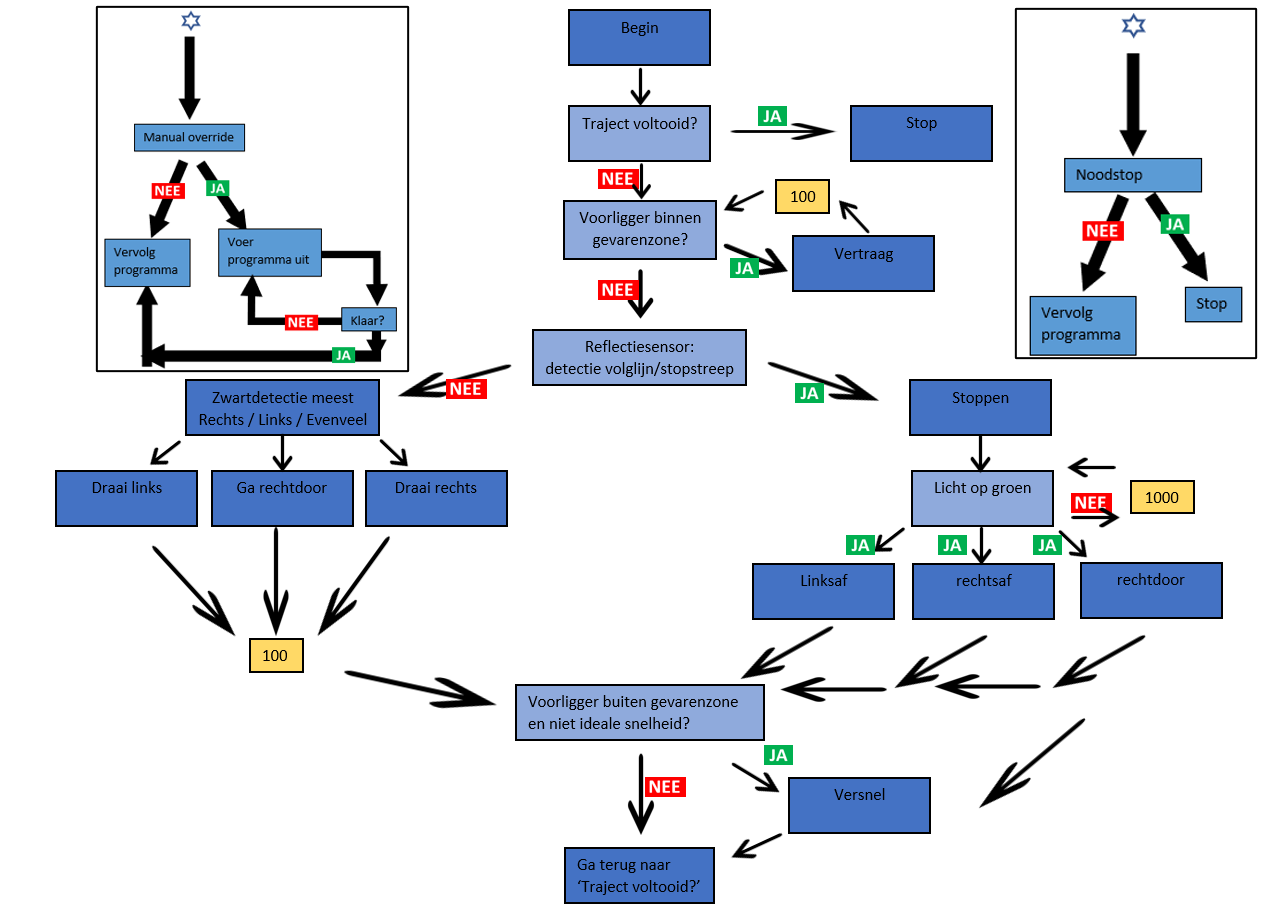
\includegraphics[width=1.3\textwidth]{fchart}
	\caption{De flowchart van ons algoritme. 
	}
	\label{fig: fchart}
	
\end{figure}

\newpage
	\section{Financieel Rapport}
	\label{sec: finrap}
	\subsection*{Hardware}
	
	\begin{table}[h]
		
	
	\begin{tabular}{l|r|r|r}
		Onderdeel& prijs per stuk & aantal & totale prijs \\
		\hline
		Micro Metal Gear Motor 100:1 HP&160 & 2 & 320 \\ 
		
		Dual Drive DRV8833 & 70 & 1 & 70 \\
		Optische afstandsensor (analoog) & 160 & 1 & 160 \\
		TCS34725 Kleur sensor BOB & 150 & 1 & 150 \\
		QTR-8A analoge reflectie sensor array & 150 & 1 & 150 \\
		Oplaadbare LITHIUM-ION & 90 & 2 & 180 \\
		NI MyRio  & 240 & 1 & 240 \\
		Breadboard Tiny & 40 & 1 & 40 \\
		Printplaat & 50 & 1 & 50 \\
		Totaal: 1360
	\end{tabular}
\caption{uitgaven hardware}
\label{tab: ess}
\end{table}
	
	
	\subsection*{Ontwerp}
\begin{table}[h]	
	\begin{tabular}{l|r|r|r}
		
		Onderdeel& prijs per stuk & aantal & totale prijs \\
		\hline
		Ball Caster &60 & 1 & 60 \\
		Wiel 60x8mm zwart &35 & 2 & 70 \\
		Robot Chassis Rechthoekig Zwart &70 & 1 & 70 \\
		
	\end{tabular}
	

	Totaal: 200
	
\caption{uitgaven ontwerp}
\label{tab: ontw}
\end{table}
	
	
	\subsection*{Assemblage}
\begin{table}[h]	
	\begin{tabular}{l|r|r|r}
		Onderdeel& prijs per stuk & aantal & totale prijs \\
		\hline
		Micro metal gear motor beugel &2 & 25 & 50 \\
		Skelet van de wagen &N.A & 1 & N.A\\
		Reflectie sensor houder &N.A & 1 & N.A\\
		
	\end{tabular}
	
	Totaal: 50
	
\caption{uitgaven assemblage}
\label{tab: ass}
\end{table}
	\subsection*{Onkosten}

\begin{table}[h]

	\begin{tabular}{l|r}
		kost& waarde \\
		\hline
		Bieding &1300 \\
		
		
	\end{tabular}
	\newline
	Totaal: 1300
\caption{uitgaven onkosten}
\label{tab: onk}
\end{table}
	
	\subsection*{Niet gebruikt}
	Totaal: 590
	
\begin{figure}[h]
	\centering
	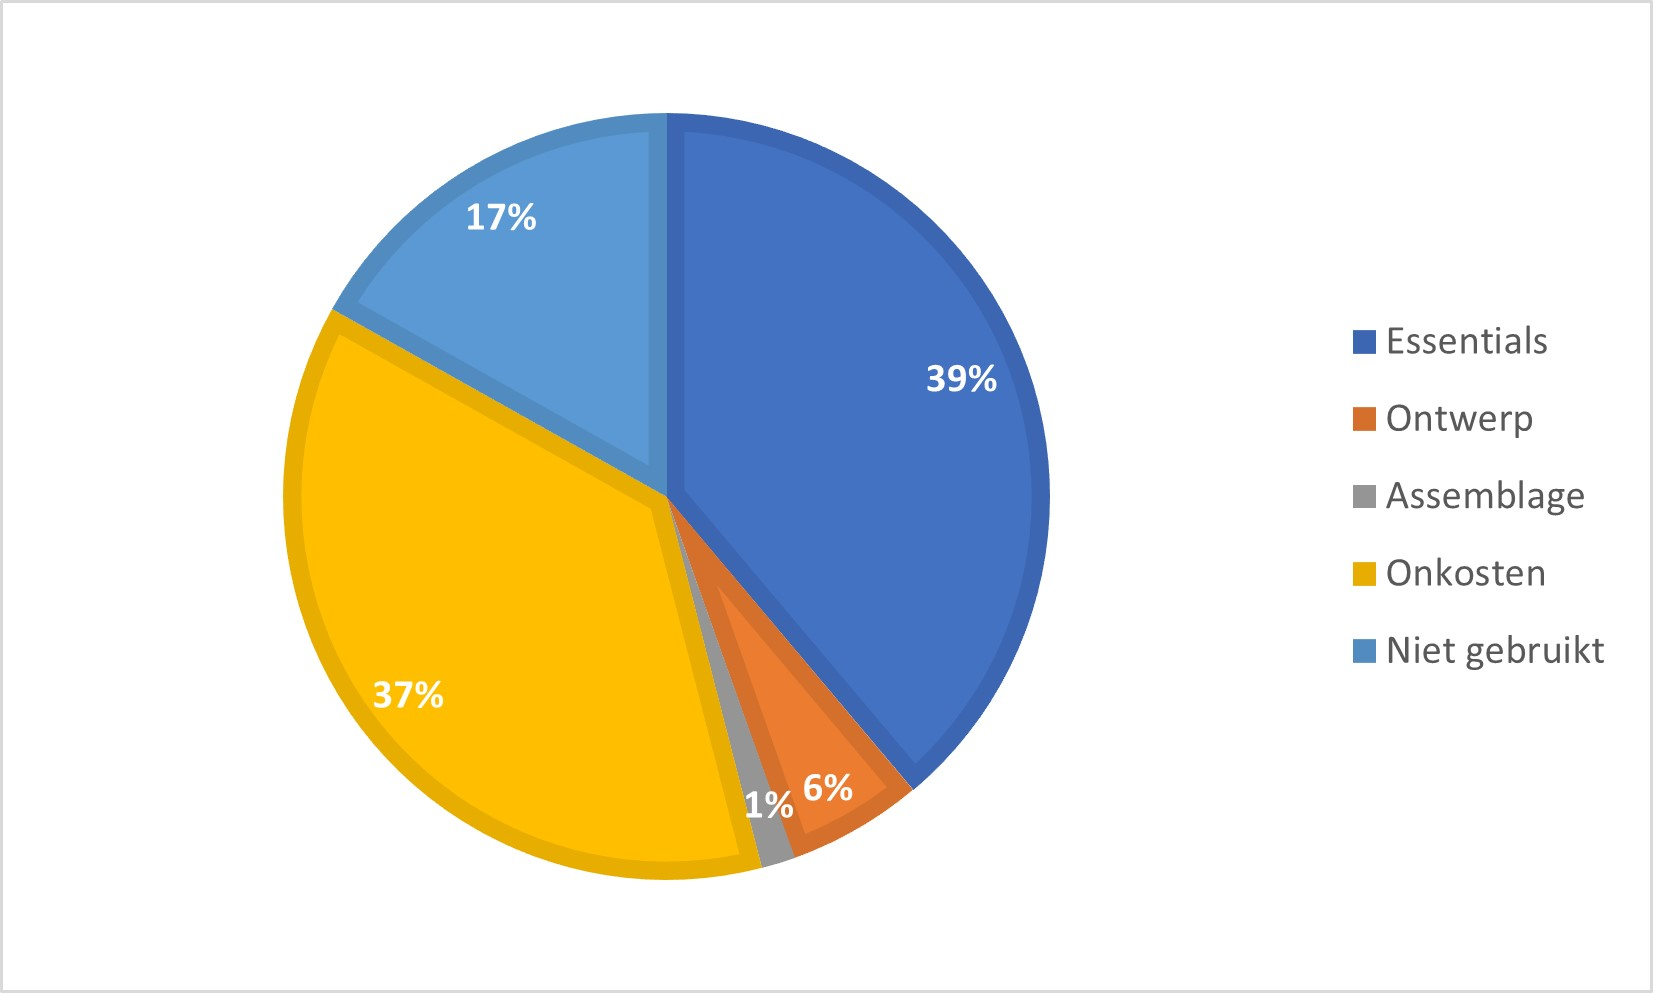
\includegraphics[width=1.2\textwidth]{pie}
	\caption{Visualisatie van de besteding van ons budget }
	\label{fig: pie}
\end{figure}
	
	
	
	
	
	
	
	%%referenties
	\bibliography{bibliografie_verslag.bib}
	\bibliographystyle{unsrt}
	
	
	
	%%Bijlagen
	
\end{document}